\documentclass[11pt,english,a4paper]{article}

\usepackage[utf8]{inputenc}          % Allows UTF-8 encoded characters in the .tex-file.
\usepackage{babel,csquotes,textcomp} % Set LaTeX to structure the content following international academic standards.
\usepackage[titletoc,toc]{appendix}
\usepackage{subfig}

\usepackage{hyperref}
\usepackage{graphicx}
\usepackage{pdfpages}
\usepackage{listings}
\usepackage{wrapfig}
\usepackage{color,colortbl}
\usepackage{lettrine}
\usepackage[font={small,it}]{caption}
\usepackage{multirow}
\usepackage{tabularx}
\usepackage{footnote}
\usepackage{enumitem}
\usepackage{amsmath}

\usepackage{setspace}
\onehalfspacing

\usepackage[
    backend=biber,
    style=numeric
]{biblatex}
\addbibresource{refs.bib}

\lstset{ %
  basicstyle=\ttfamily\small,     
  backgroundcolor=\color{white},   % choose the background color
  breaklines=true,                 % automatic line breaking only at whitespace
  captionpos=b,                    % sets the caption-position to bottom
  commentstyle=\color{mygreen},    % comment style
  escapeinside={\%*}{*)},          % if you want to add LaTeX within your code
  keywordstyle=\color{blue},       % keyword style
  stringstyle=\color{mymauve},     % string literal style
}

\title{Lab report \\ GPSDO}
\author{Aril Schultzen}

\begin{document}
\maketitle
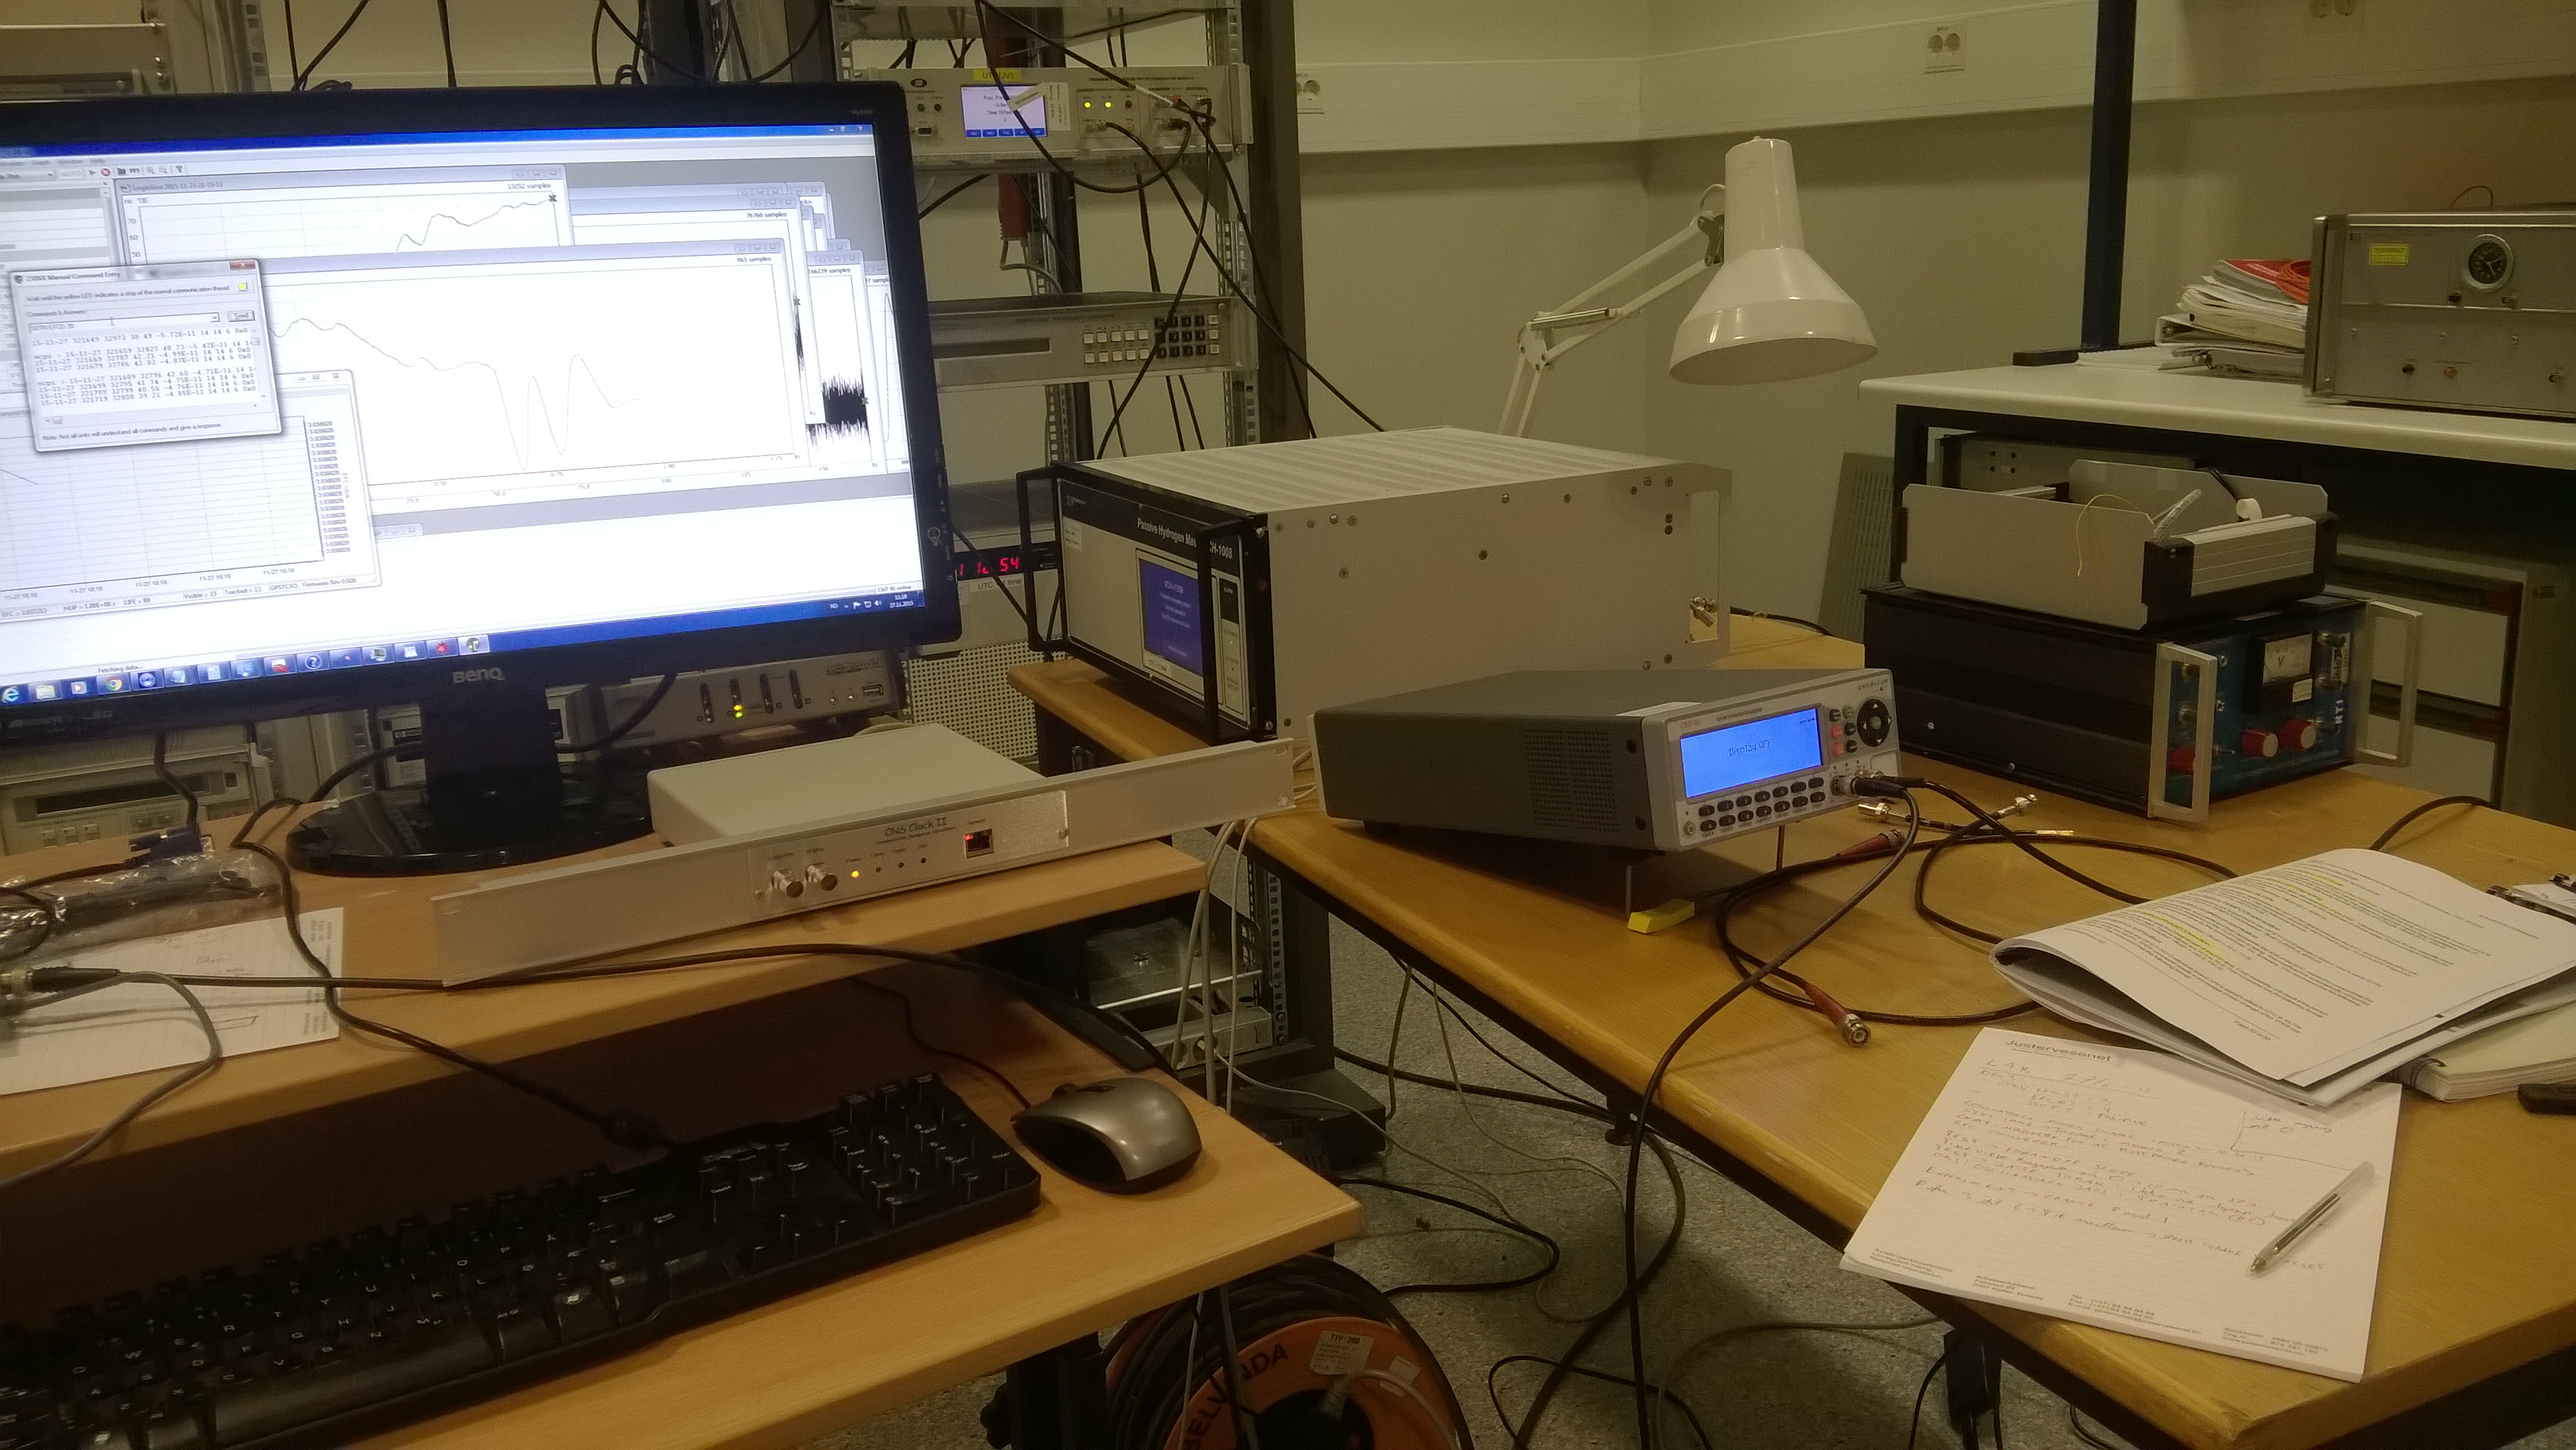
\includegraphics[width=1 \textwidth]{lab.jpg}
\section{Objective}
\begin{itemize}
\item Gain knowledge and understanding of the properties of GPS disciplined oscillator
\item Receive further training in the use of frequency counters as well as tools used to analyze frequency stability.
\end{itemize}

\section{Equipment}
\begin{itemize}
  \item Jackson Labs GPS-300 v1.0 Prototype
  \item PHM, Passive Hydrogen maser, frequency reference
  \item Pendulum CNT-91, Frequency counter
  \item Tektronix MD0-4000-6 Oscilloscope
  \item Z38XX Software
  \item TimeView
  \item TimeLab
\end{itemize}

\section{Before the lab}
\begin{itemize}
  \item The GPS-300 was started in advance and had GPS lock for a minimum of 12 hours.
  \item Z3800X was started and configured to store all log data to the applications root folder with the following format for files: \newline \texttt{Z38XX<YEAR>W<WEEK\_NR>.txt}
  \item A TIE measurement was conducted spanning over 10 hours using the CNT-91 as counter with the maser as reference.
\end{itemize}

\section{Part 1: GPS disciplined oscillator}
\begin{figure}[!htb]
  \centering
  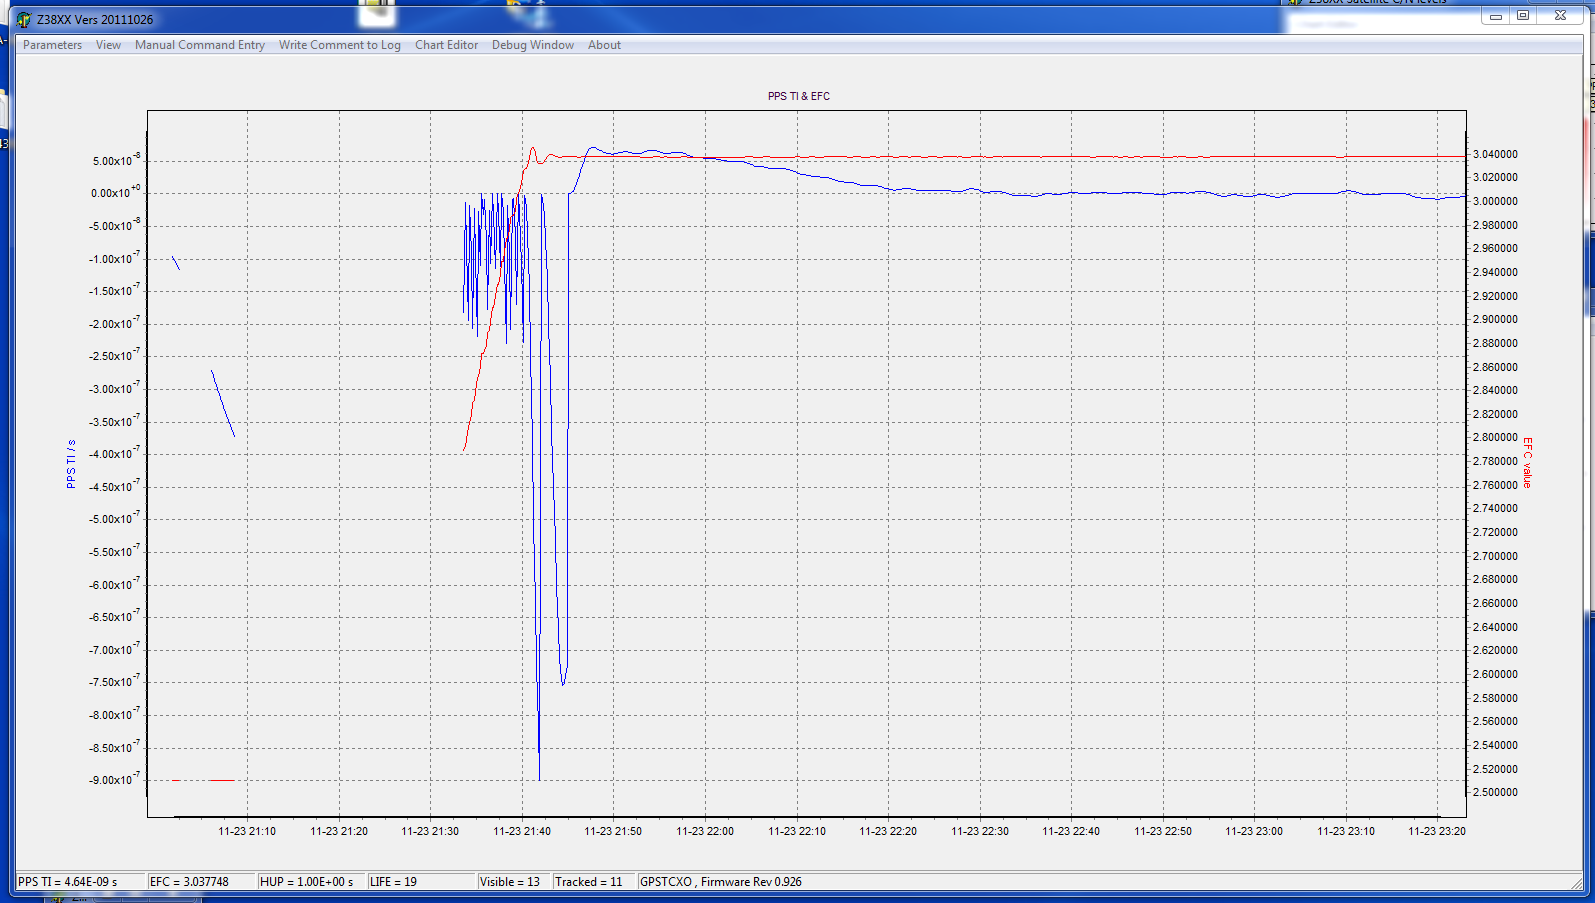
\includegraphics[width=1\textwidth]{z38xx_EFC_oppstart.PNG}
  \caption[Z38XX screen shot] {The figure above shows a screen shot from the Z38XX software. The oscillator is all warmed up and ready to go.} 
  \label{fig:z38xx_oppstart}
\end{figure}

\subsection{Observations}
Figure \ref{fig:z38xx_oppstart} shows that the GPS receiver on the GPS-300 has a total of 13 satellites visible and that it is currently tracking 11, which is more than sufficient for timing purposes. It is also reasonable to assume that it has finished warming up considering how dramatic the readings where and how they are now. 

\begin{figure}[!htb]
  \centering
    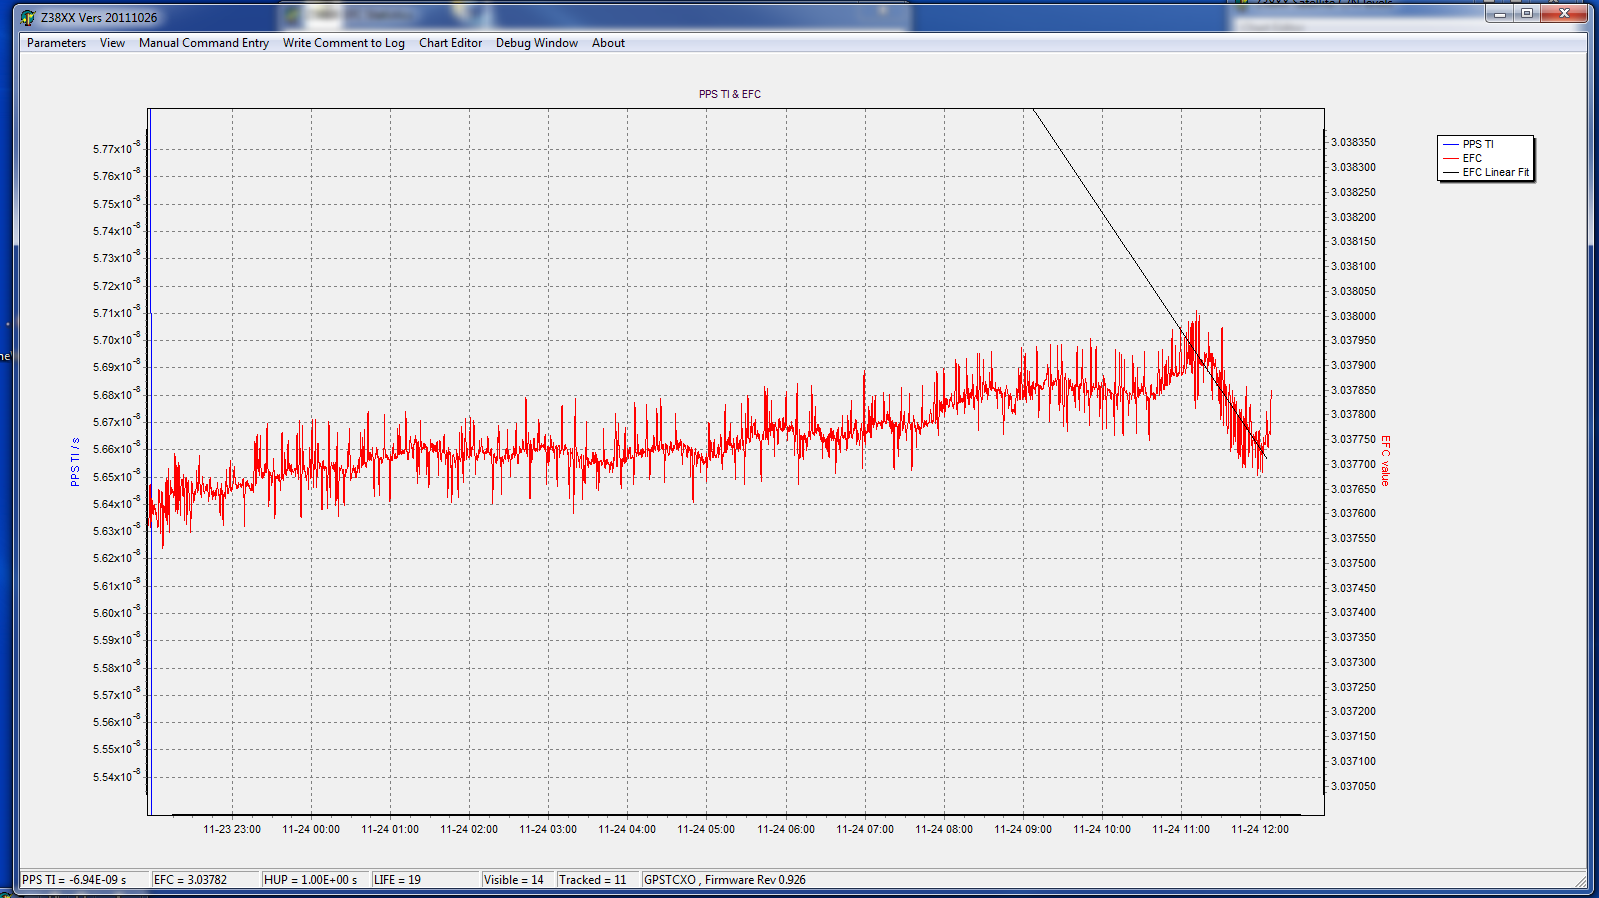
\includegraphics[width=1\textwidth]{z38xx_EFC_oppvarmet_zoom.PNG}
      \caption{Screenshot of Z38XX showing all the collected data, including the warm-up.}
      \label{fig:Z38XX_gpsdo12}
\end{figure}

\begin{figure}[!htb]
  \centering
    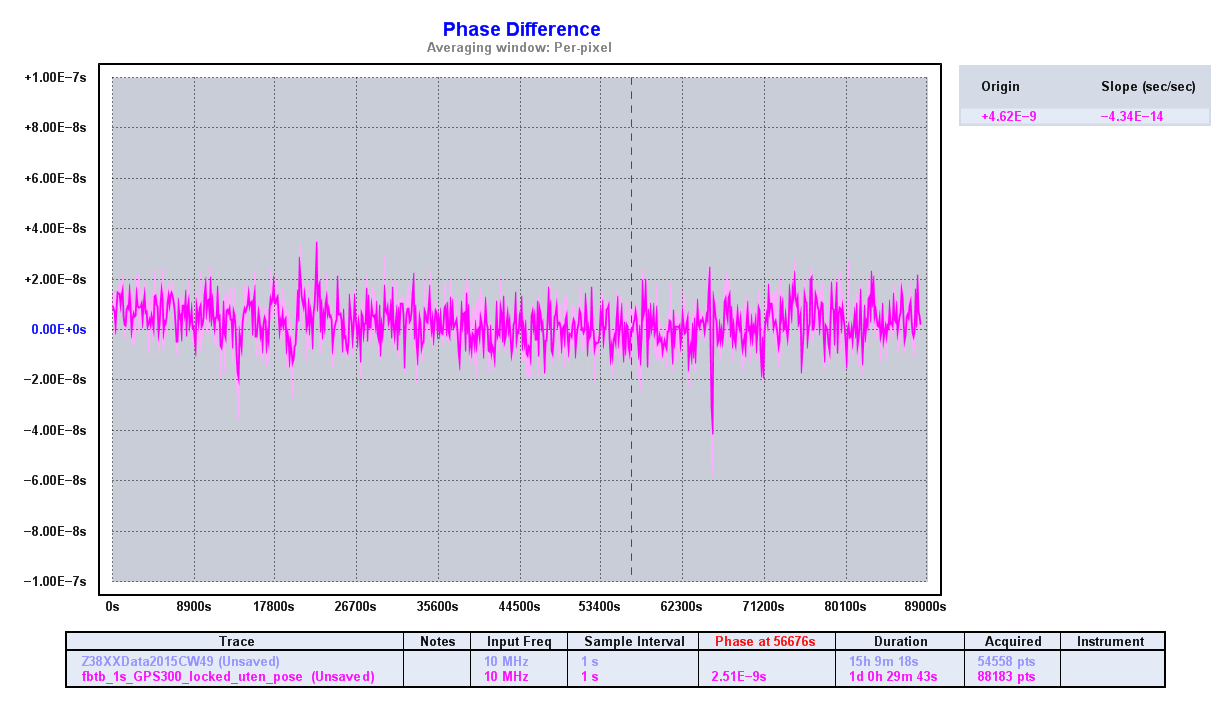
\includegraphics[width=1\textwidth]{part1_spm3_fbtb_phase_diff.png}
      \caption{Phase difference for the GPS-300 measured using the CNT-91 counter}
          \label{fig:part1_spm3_fbtb_phase_diff}
\end{figure}

\begin{figure}[!htb]
  \centering
    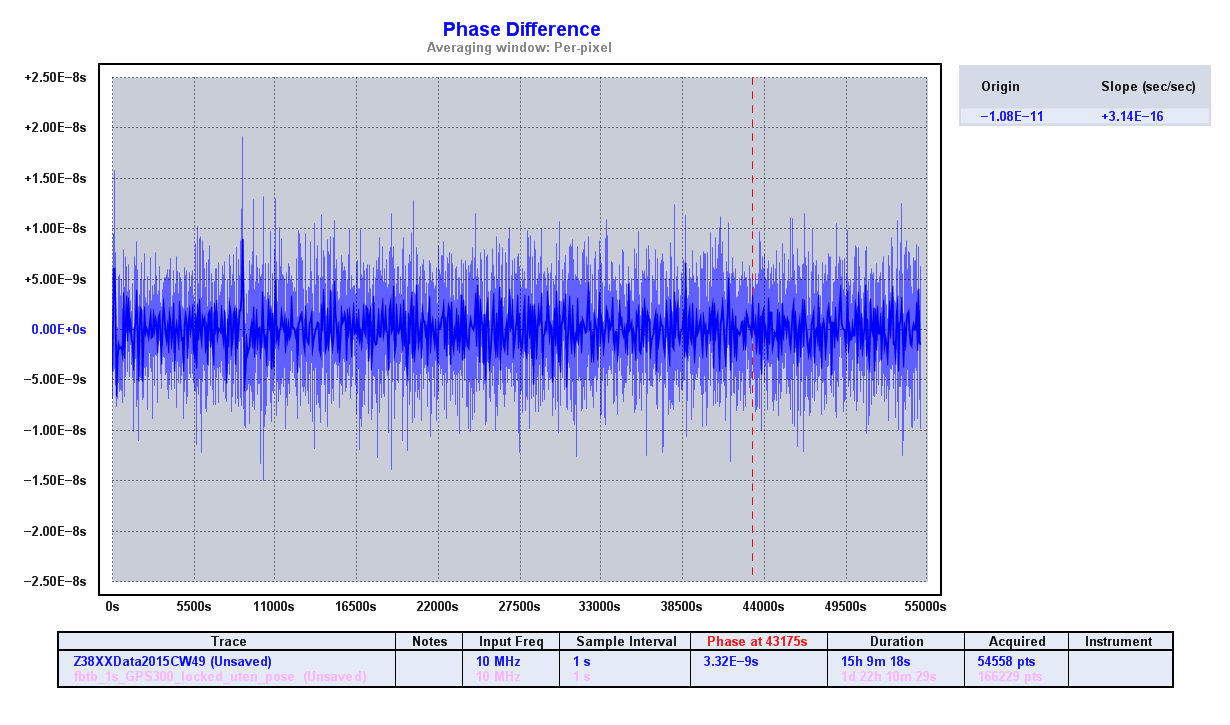
\includegraphics[width=1\textwidth]{part1_spm3_x38_phase_diff.png}
      \caption{Phase difference for the GPS-300 measured using the internal counter}
          \label{fig:part1_spm3_x38_phase_diff}
\end{figure}

When comparing the figure \ref{fig:part1_spm3_fbtb_phase_diff} showing phase difference from a frequency back-to-back  measurement done with our setup and figure \ref{fig:part1_spm3_x38_phase_diff} showing the phase difference measured by the internal counter on the GPS-300, it becomes obvious that the counter on the GPS-300 board is less accurate than our setup and therefore measures a little optimistic. The reason is that it has got a completely different and better reference. The CNT-91 timer uses the PHM as a reference while the GPS-300 uses GPS. GPS signals are extremely noisy compared to a PHM. The timer on the GPS-300 is also likely sub-par compared to the CNT-91. 

\begin{figure}[!htb]
  \centering
    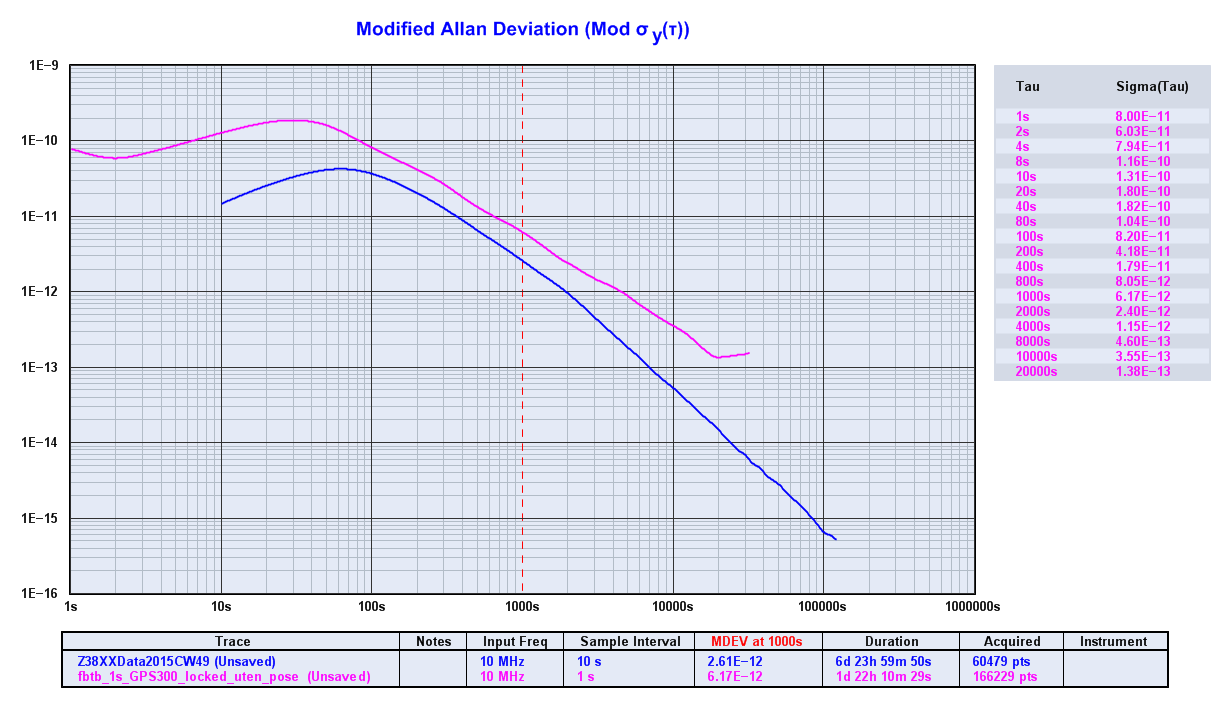
\includegraphics[width=1\textwidth]{part1_spm4_modified_allan.png}
      \caption{Modified Allan Deviation for GPS-300 measured by the internal counter (pink) and CNT-91 (blue))}
          \label{fig:part1_spm4_modified_allan}
\end{figure}

\begin{figure}[!htb]
  \centering
    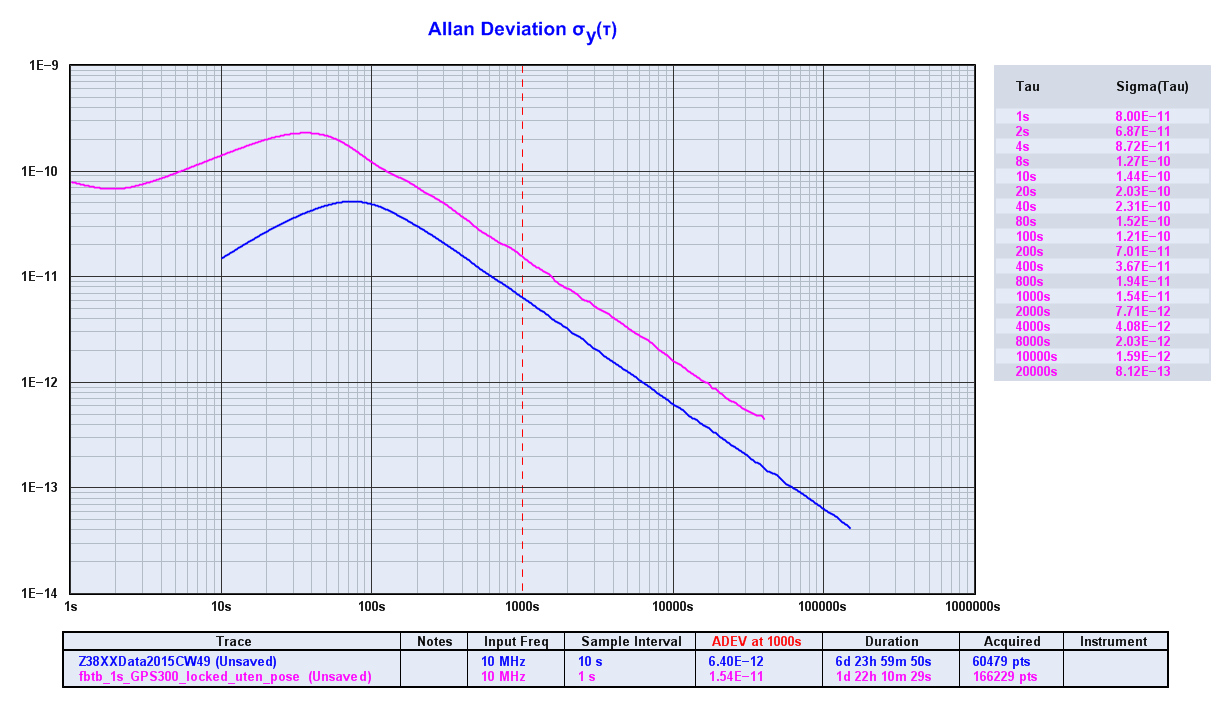
\includegraphics[width=1\textwidth]{part1_spm4_allan.png}
      \caption{Allan Deviation for GPS-300 measured by the internal counter (pink) and CNT-91 (blue)}
          \label{fig:part1_spm4_allan}
\end{figure}

\begin{figure}[!htb]
  \centering
    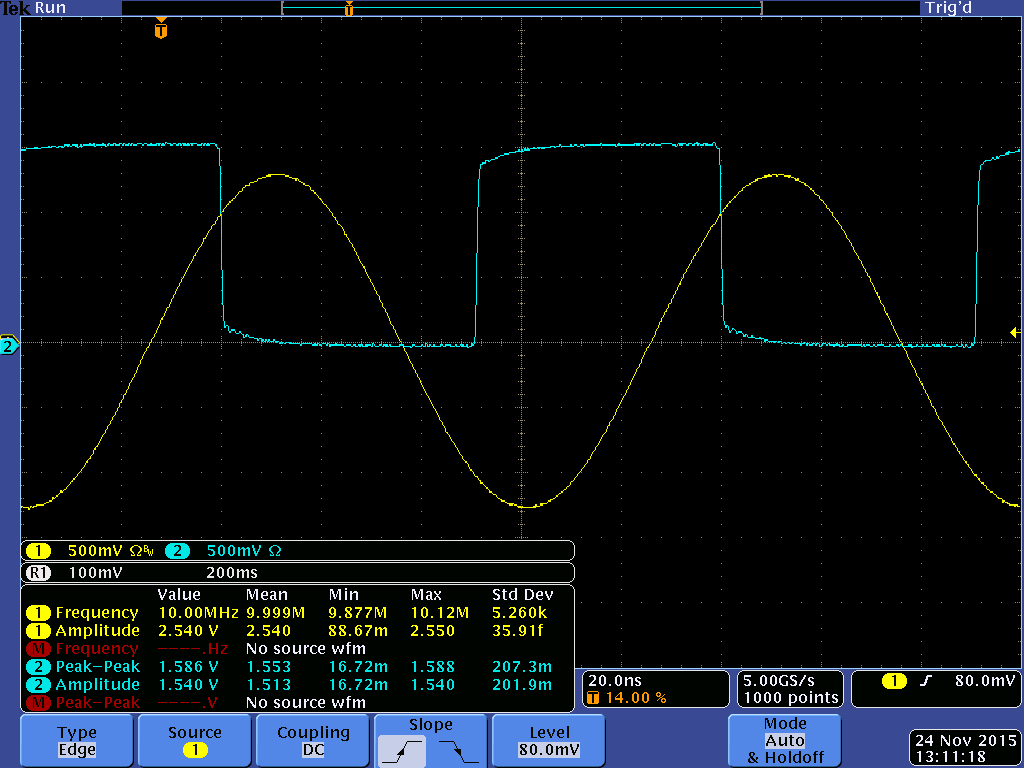
\includegraphics[width=1\textwidth]{tek00006.png}
      \caption{screenshot from the oscilloscope and shows both the GPS-300 and the PHM, trigging at the PHM (yellow)}
          \label{fig:tek00006}
\end{figure}

\begin{figure}[!htb]
  \centering
    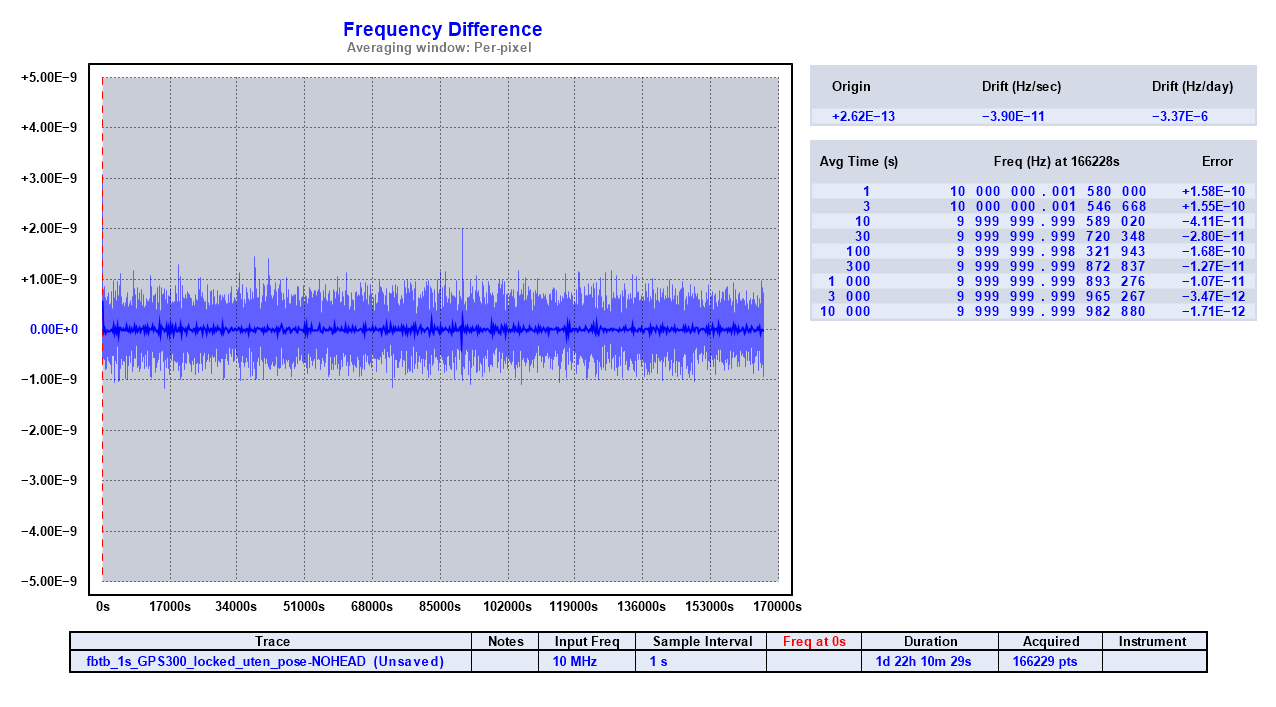
\includegraphics[width=1\textwidth]{part1_spm5_freq_diff.png}
      \caption{GPS-300 1s sample rate frequency back-to-back, frequency difference}
          \label{fig:part1_spm5_freq_diff}
\end{figure}

\newpage
When comparing the measurement done by GPS-300's internal counter with our setup in the context of both regular (figure \ref{fig:part1_spm4_modified_allan}) and Modified Allan Deviation (figure \ref{fig:part1_spm4_allan}), it's clear that the measurement on our setup is the correct one. 

% spm5 %
Figure \ref{fig:tek00006} is a screenshot of the oscilloscope and shows both the GPS-300 and the PHM, trigging at the PHM (yellow). Upon observation of the oscilloscope, a PID like oscillation effect could be observed. When studying the figure \ref{fig:part1_spm5_freq_diff} showing the frequency difference made from a measurement done with our setup, this effect becomes more visible. One way to picture it, is that movement along the X-axis on the oscilloscope correlates to "movement" along the the Y-axis on figure \ref{fig:part1_spm5_freq_diff}. 

% spm6 %

\newpage
Figure \ref{fig:del_1_spm6_mod_allan} and \ref{fig:del_1_spm6_allan} shows the Modified and regular Allan Deviation for three measurements all done with our setup:
\begin{itemize}
  \item TIE 100$\mu$s sample rate, PHM (light-blue)
  \item TIE 100$\mu$s sample rate, GPS-300 in holdover mode (red)
  \item TIE 100$\mu$s sample rate, GPS-300 in locked (GPS disciplined mode) smoothed over 1000 points (green)
\end{itemize}
Because of the 1000 point smoothing (green), not much can be said about the stability before 0.1 s. When comparing with the plot for the PHM, it becomes clear that any instability after 0.1 s is not because of the measurement setup, but rather the oscillator itself. However, by using the smoothing method, we are able to obtain resolution that would not be possible because of limitations in the measuring setup, already at 0.1 s instead of $approx$1.6s. By looking at the Modified Allan Deviation for the PHM, the limit of what you could hope to achieve in terms of resolution is revealed. This is because of how the Modified Allan Deviation is calculated by using a running average. This is also what makes it possible to separate white noise from flicker noise since white noise is uncorrelated and therefore possible to reduce by calculating an average.   

Comparing with Symmetricom's own Allan Deviation, the GPS-300 actually performs better than their estimation. At 1 s, we measured 4.42E-11 as opposed to $\approx$ 9.00E-11. At 10 s, we measured 5.20E-11 and they $\approx$6.00E-10.

\begin{figure}[!htb]
  \centering
    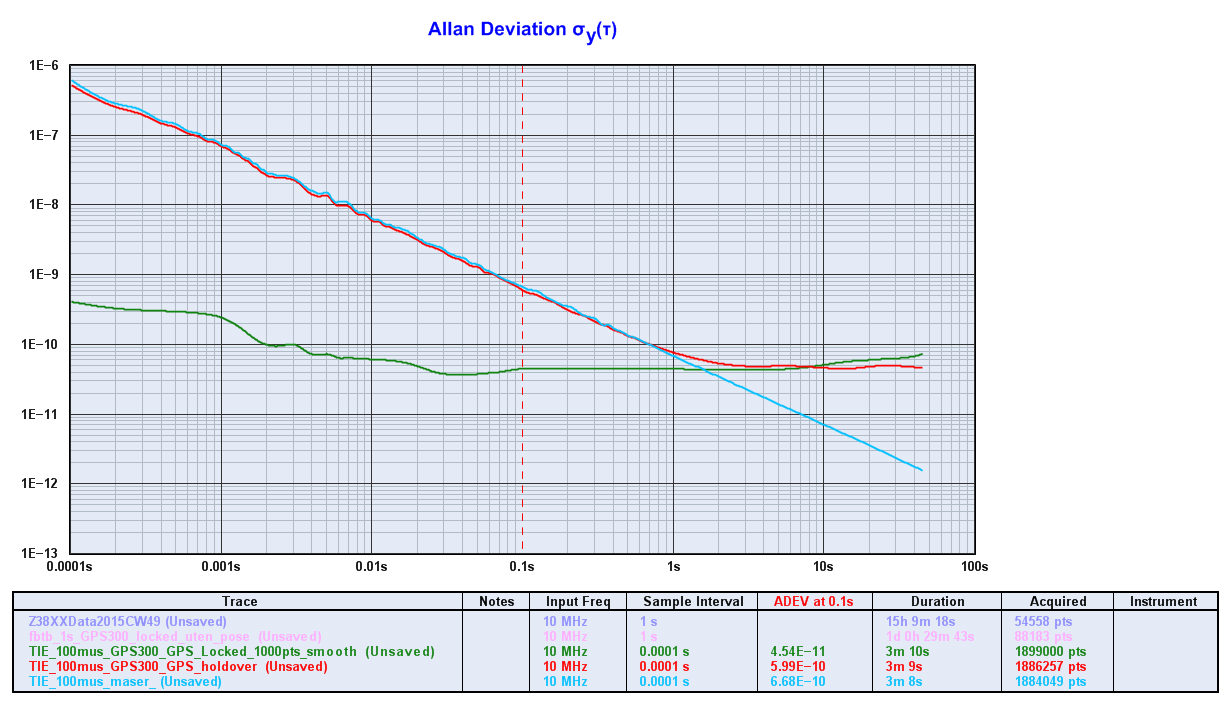
\includegraphics[width=1\textwidth]{del_1_spm6_allan.png}
      \caption{Allan Deviation. TIE 100$\mu$s for GPS-300 in both Locked (green), Holdover (red) and PHM (light-blue). The measurement for Locked GPS-300 is smoothed over 1000 pts.}
          \label{fig:del_1_spm6_allan}
\end{figure}

\begin{figure}[!htb]
  \centering
    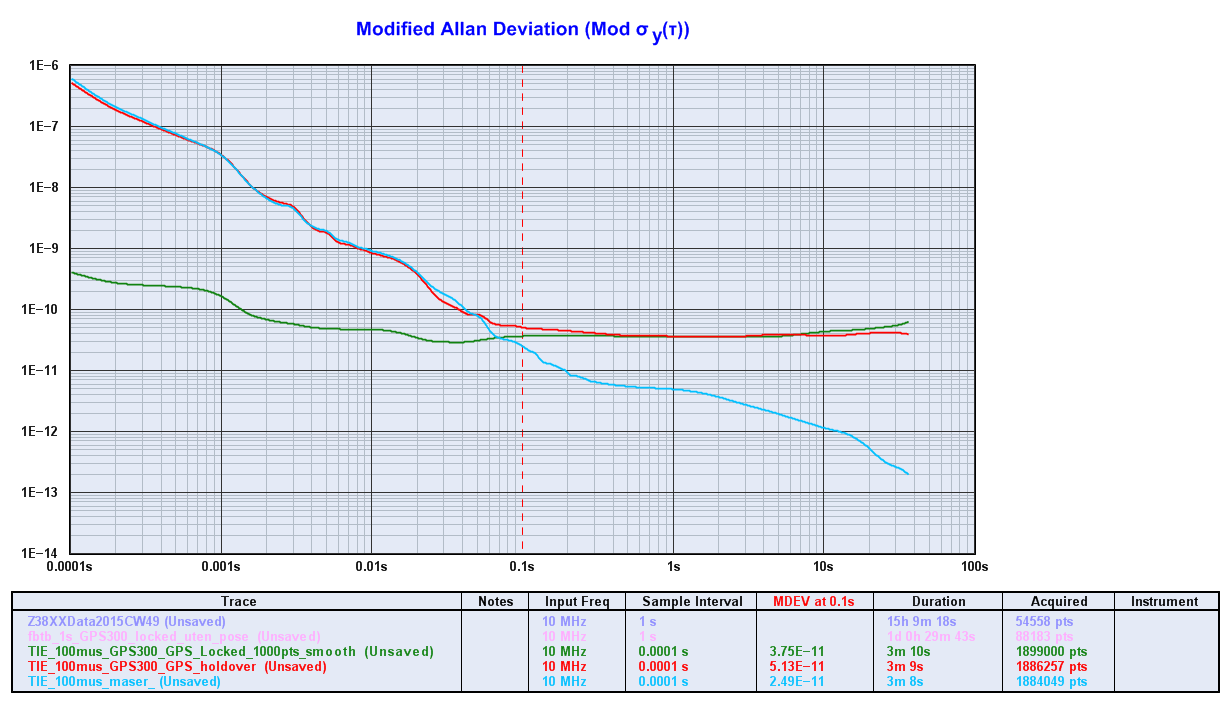
\includegraphics[width=1\textwidth]{del_1_spm6_mod_allan.png}
      \caption{Modified Allan Deviation. TIE 100$\mu$s for GPS-300 in both Locked (green), Holdover (red) and PHM (light-blue). The measurement for Locked GPS-300 is smoothed over 1000 pts}
          \label{fig:del_1_spm6_mod_allan}
\end{figure}

\section{Part 2: Free-range oscillator}

\begin{figure}[!htb]
  \centering
    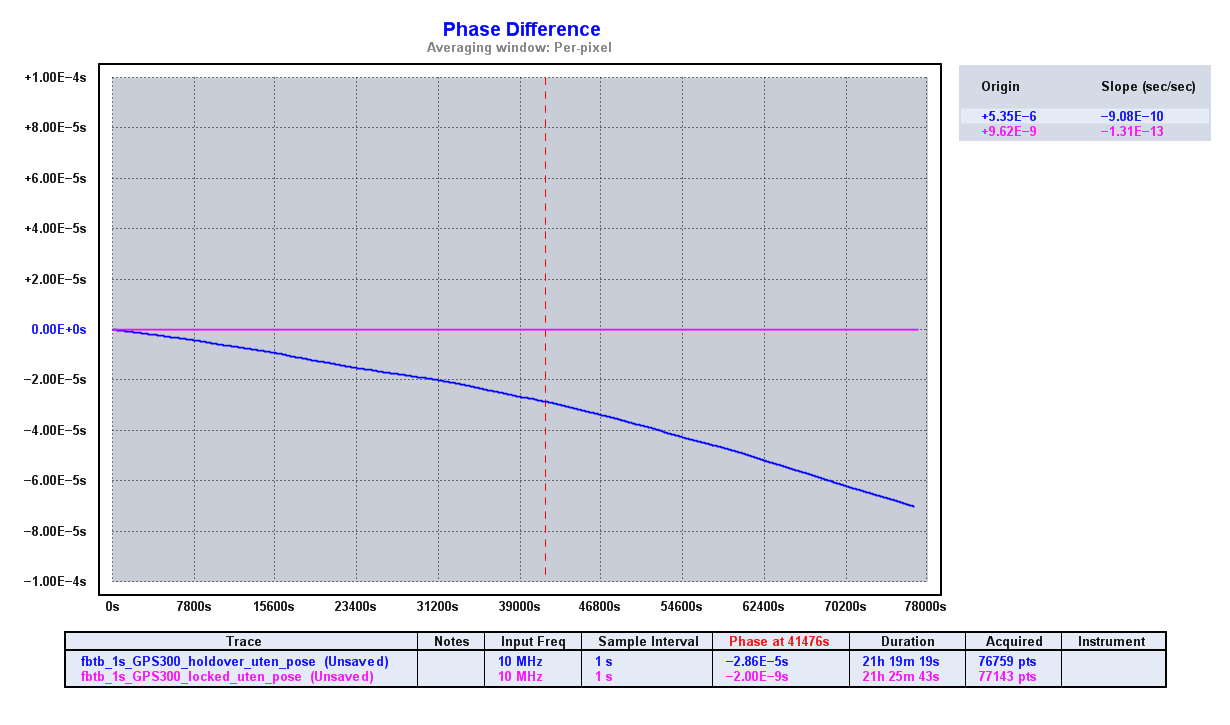
\includegraphics[width=1\textwidth]{del_2_spm1_phase_diff.png}
      \caption{FBTB 1 s, Phase difference for GPS-300 during holdover mode (blue) and locked mode (pink).}
          \label{fig:del_2_spm1_phase_diff}
\end{figure}

\begin{figure}[!htb]
  \centering
    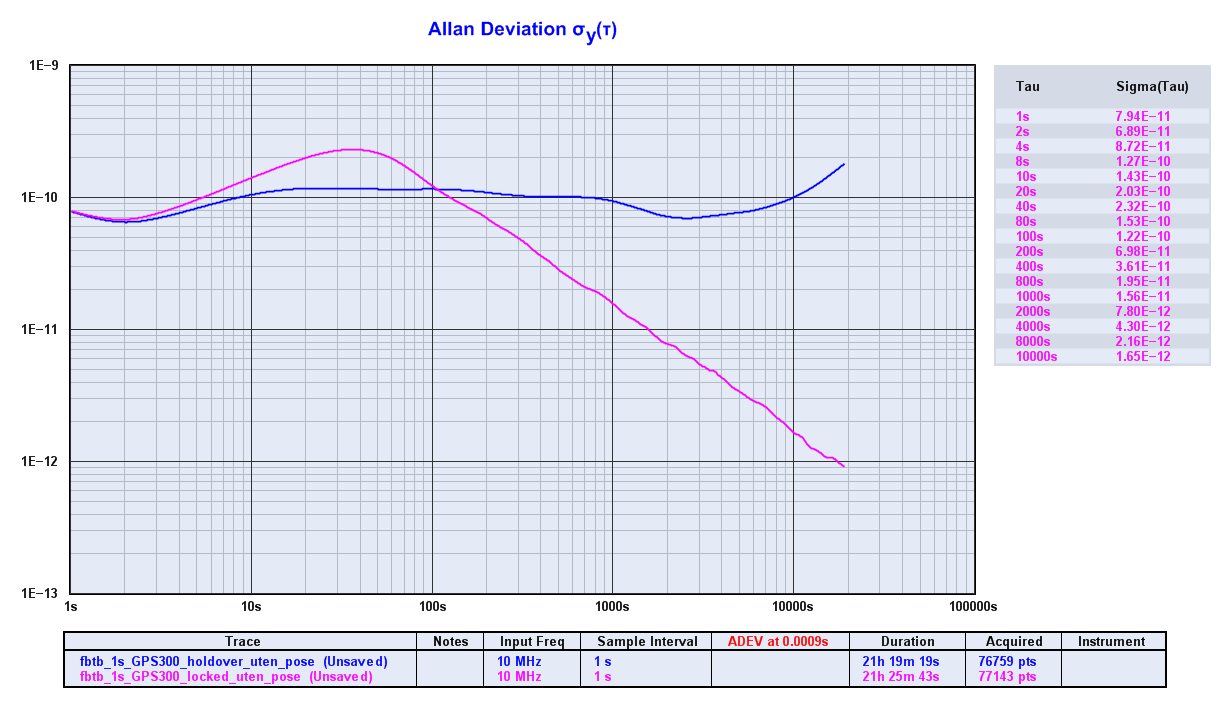
\includegraphics[width=1\textwidth]{del_2_spm1_allan_dev.png}
      \caption{FBTB 1 s, Allan Deviation for GPS-300 during holdover mode (blue) and locked mode (pink).}
          \label{fig:del_2_spm1_allan_dev}
\end{figure}
When comparing the Allan Deviation for the measurement taken with and without GPS lock (figure \ref{fig:del_2_spm1_allan_dev}), one can observe that the long term stability is better when in locked mode. This is not a surprise, but when observing the plot for the oscillator when in Holdover mode, one can see that the short term stability is better than when disciplined. One could perhaps argue that the oscillator stability in locked mode would benefit from a longer time constant (between GPS synch), but this depends on the temperature variations of the environment of which it is operating. In the lab where this experiment was exercised, the temperature is much more stable than one could hope to encounter "in the wild".
\end{document}                     